\section{Part I: Analysis of Bandit Algorithms}

(1) Reproduce the proof for Regret Decomposition Lemma

(2) Given $k$ actions, we define a preference function $H(\cdot):\{1, \ldots, k\} \rightarrow \mathcal{R}$. Then for actions $x\in\{1, \ldots, k\}$ and $y\in\{1, \ldots, k\}$, we define a soft-max function
$$\pi(x)=\dfrac{e^{H(x)}}{\sum_{y=1}^k e^{H(y)}}$$
Please show the following result: for any action $a\in\{1, \ldots, k\}$, we have
$$\dfrac{\partial \pi(x)}{\partial H(a)}=\pi(x)\left(\I_{(x=a)}-\pi(a)\right)$$
where $\I_A$ is an index function of events, being 1 when event $A$ is true and being 0 otherwise.

(3) Reproduce the proof for gradient bandit algorithm.

(4) (Bouns): show the proof for the regret upper bound of UCB1 algorithm

(5) (Bonus): show the proof for the regret upper bound of Thompson sampling algorithm (Beta-Bernoulli bandit only)

\solution

(1) Let $a_{\tau}$ be a random variable representing to the $\tau$-th action, and $r_{\tau}$ be the reward, which is also a random variable. Since $a_{\tau}$ is a random variable, so $Q(a_\tau) = \E_{r_{\tau}}[r_\tau | a_\tau]$ is also a random variable of $a_{\tau}$, and according to Adam's rule, we can get that:
$$\E_{a_{\tau}}[Q(a_\tau)] = \E_{a_{\tau}}[\E_{r_{\tau}}[r_\tau | a_\tau]] = \E\left[r_\tau\right]$$
Define the total expected reward $S_t = \sum\limits_{\tau=1}^{t}Q(a_\tau)$, then we have:
$$\E(S_t) = \E\left[\sum_{\tau=1}^{t} Q(a_\tau)\right] = \sum_{\tau=1}^{t}\E\left[ Q(a_\tau)\right] = \sum_{\tau=1}^{t}\E\left[r_\tau\right] = \E\left[\sum_{\tau=1}^{t}r_\tau\right] $$
Since for each step, an arm must be pulled, so let $\A$ be the action space, then $\forall \tau, \sum\limits_{a\in\A}\I_{a_\tau = a} = 1$, thus:
\begin{equation}
\begin{aligned}
\E(S_t) & = \E\left[\sum_{\tau=1}^{t}r_\tau\right] \\
&=  \E\left[\sum_{\tau=1}^{t}\sum_{a\in\A}r_\tau \I_{a_\tau = a}\right] \\
&=  \sum_{a\in\A}\sum_{\tau=1}^{t}\E\left[r_\tau \I_{a_\tau = a}\right]
\end{aligned}
\end{equation}
On the other hand, for $t$ steps, the arms are pulled totally $t$ times, thus
\begin{equation}
\begin{aligned}
&\qquad\ \sum_{\tau=1}^{t}\sum_{a\in\A}\I_{a_\tau = a} = \sum_{\tau=1}^{t} 1 = t \\
&\Rightarrow \E\left[\sum_{\tau=1}^{t}\sum_{a\in\A}\I_{a_\tau = a}\right] = t \\
&\Rightarrow \sum_{\tau=1}^{t}\sum_{a\in\A}\E\left[\I_{a_\tau = a}\right] = t \\
&\Rightarrow \sum_{a\in\A}\sum_{\tau=1}^{t}\E\left[\I_{a_\tau = a}\right] = t
\end{aligned}
\end{equation}
Define $V^*$ be the expected reward of the best action, i.e. $V^*=\max\limits_{a\in\A}Q(a)$, and according to the definition of each action's regret, we have
$$L_{\tau}=\E_{a_{\tau}}\left[V^*-Q(a_{\tau})\right]$$
So the total regret is
\begin{equation}
\begin{aligned}
L_t &= \sum_{\tau=1}^{t}\E_{a_{\tau}}\left[{V^{*} - Q(a_\tau)}\right] \\
&= tV^* - \E\left[\sum_{\tau=1}^{t}Q(a_\tau)\right] \\
&= tV^* - \E(S_t)\\
&\stackrel{(1),(2)}{=} \sum_{a\in\A}\sum_{\tau=1}^{t}\E\left[\I_{a_\tau = a}\right]V^* - \sum_{a\in\A}\sum_{\tau=1}^{t}\E\left[r_\tau \I_{a_\tau = a}\right] \\
&= \sum_{a\in\A}\sum_{\tau=1}^{t}\E\left[(V^* - r_\tau)\I_{a_\tau = a}\right]
\end{aligned}
\end{equation}
Let $\Delta_a$ be the gap between the expected reward between the best action and action $a$, i.e. $\Delta_a = V^* - Q(a)$, then we have:
\begin{align*}
&\quad\ \E\left[(V^* - r_\tau)\I_{a_\tau = a} | a_\tau\right] \\
&= \I_{a_\tau = a}\E\left[(V^* - r_\tau) | a_\tau\right] \\
&= \I_{a_\tau = a}(V^* - Q(a_{\tau})) \qquad\text{(Definition of $Q(a_{\tau}$))} \\
&= \I_{a_\tau = a}(V^* - Q(a)) \\
&= \I_{a_\tau = a}\Delta_a
\end{align*}
Using Adam's low, we can get that
\begin{equation}
\E\left[(V^* - r_\tau)\I_{a_\tau = a}\right] = \E_{a_{\tau}}\left[\E\left[(V^* - r_\tau)\I_{a_\tau = a} | a_\tau\right]\right] = \E_{a_{\tau}}\left[\I_{a_\tau = a}\Delta_a\right]
\end{equation}
Define the number of action $a$ is selected after $t$ steps as $N_t(a)$, and let $\pi$ be the policy, then the total regret is:
\begin{align*}
L_t &\stackrel{(3)}{=} \sum_{a\in\A}\sum_{\tau=1}^{t}\E\left[(V^* - r_\tau)\I_{a_\tau = a}\right] \\
&\stackrel{(4)}{=} \sum_{a\in\A}\sum_{\tau=1}^{t}\E\left[\I_{a_\tau = a}\Delta_a\right] \\
&= \sum_{a\in\A}\E\left[\sum_{\tau=1}^{t}\I_{a_\tau = a}\right]\Delta_a \\
&= \sum_{a\in\A}\E_{\pi}\left[N_t(a)\right]\Delta_a
\end{align*}
So above all, we have proved the regret decomposition lemma:
$$L_t = \sum_{a\in\A}\E_{\pi}\left[N_t(a)\right]\Delta_a$$

(2) Since the distribution is the softmax function
$$\pi(x) = \dfrac{e^{H(x)}}{\sum_{y=1}^{k} e^{H(y)}}$$
Then we can get that
\begin{equation}
\begin{aligned}
\dfrac{\partial{\pi(x)}}{\partial{H(a)}} &= \dfrac{\partial{\frac{e^{H(x)}}{\sum_{y=1}^{k}{e^{H(y)}}}}}{\partial{H(a)}} \\
&= \dfrac{\frac{\partial{H(x)}}{\partial{H(a)}}\cdot\left(\sum_{y=1}^{k}{e^{H(y)}}\right) -e^{H(x)}\cdot e^{H(a)}}{\left(\sum_{y=1}^{k}{e^{H(y)}}\right)^2} \\
&= \dfrac{\I_{x=a}e^{H(x)}\cdot\left(\sum_{y=1}^{k}{e^{H(y)}}\right) -e^{H(x)}\cdot e^{H(a)}}{\left(\sum_{y=1}^{k}{e^{H(y)}}\right)^2} \\
&= \dfrac{e^{H(x)}}{\sum_{y=1}^{k}{e^{H(y)}}}\left(\I_{x=a} - \dfrac{e^{H(a)}}{\sum_{y=1}^{k}{e^{H(y)}}}\right) \\
&= \pi(x)\left(\I_{x=a} - \pi(a)\right)
\end{aligned}
\end{equation}
So above all, we have proved that
$$\dfrac{\partial{\pi(x)}}{\partial{H(a)}} = \pi(x)\left(\I_{x=a} - \pi(a)\right)$$

(3) The objective function is $\max\ \E_{R_t}\left[R_t\right]$. Using Adam's law and LOTE, we can get that:
\begin{align*}
\E_{R_t}\left[R_t\right] &= \E_{A_t}\left[\E_{R_t}\left[R_t|A_t\right]\right] \qquad\qquad\qquad\ \ \text{(Adam's Law)} \\
&= \sum_{x}\E_{R_t}\left[R_t|A_t=x\right]P(A_t=x) \quad\text{(LOTE)} \\
&= \sum_x Q(x)\pi_t(x)
\end{align*}
where $Q(a)=\E_{R_t}\left[R_t|A_t=a\right]$ is fixed, and $\pi_t(x) \propto e^{H_t(x)}$. \\
Since $\sum\limits_x \pi_t(x) = 1$, so
\begin{equation}
\dfrac{\partial \sum_x\pi_t(x)}{\partial H_t(a)} = 0 \Rightarrow \sum\limits_x \dfrac{\partial \pi_t(x)}{\partial H_t(a)} = 0 \Rightarrow \sum\limits_x B_t\cdot \dfrac{\partial \pi_t(x)}{\partial H_t(a)} = 0
\end{equation}
Thus a baseline $B_t$, which is independent with $x$ could be added to ensure a better convergence and lower variance. Thus the derivative of $\E_{R_t}\left[R_t\right]$ becomes:
\begin{align*}
\dfrac{\partial \E_{R_t}\left[R_t\right]}{\partial H_t(a)} &= \sum_x Q(x)\dfrac{\partial \pi_t(A_t)}{\partial H_t(a)} \\
&\stackrel{(6)}{=} \sum_x \left(Q(x)\dfrac{\partial \pi_t(A_t)}{\partial H_t(a)} - B_t\cdot \dfrac{\partial \pi_t(x)}{\partial H_t(a)} \right) \\
&\stackrel{(5)}{=} \sum_x \left(Q(x)-B_t\right) \pi_t(x)\left(\I_{A_t=a} - \pi_t(a)\right) \\
&= \E_{A_t\sim\pi_t}\left[(Q(A_t)-B_t) \left(\I_{A_t=a} - \pi_t(a)\right)\right]
\end{align*}
According to the definition $Q(A_t)=\E_{R_t}\left[R_t|A_t\right]$ is a random variable, we can get that:
\begin{align*}
&\quad\ \E\left[Q(A_t) (\I_{A_t=a} - \pi_t(a))\right] \\
&= \E_{A_t\sim\pi_t}\left[\E_{R_t}\left[R_t|A_t\right] (\I_{A_t=a} - \pi_t(a))\right] \\
&= \E_{A_t\sim\pi_t}\left[\E_{R_t}\left[R_t(\I_{A_t=a} - \pi_t(a))|A_t\right]\right] \\
&= \E_{A_t\sim\pi_t}\left[R_t(\I_{A_t=a} - \pi_t(a))\right] \qquad\qquad\ \text{(Adam's Law)}
\end{align*}

So we can maximum $\E\left[R_t\right]$ by maximizing $H_t(x)$, which could use the gradient ascent methods. To save computation, using the stochastic gradient ascent method, for each iteration with step size $\alpha$, we have
\begin{align*}
H_{t+1}(a) &\gets H_t(a) +\alpha \dfrac{\partial \E_{R_t}\left[R_t\right]}{\partial H_t(a)} \\
&= H_t(a) +\alpha \E\left[(Q(A_t)-B_t) (\I_{A_t=a} - \pi_t(a))\right] \\
&= H_t(a) +\alpha \E\left[(R_t-B_t) (\I_{A_t=a} - \pi_t(a))\right] \\
&= H_t(a) +\alpha \left(R_t-B_t\right) (\I_{A_t=a} - \pi_t(a)) \qquad\text{(Stochastic gradient ascent)}
\end{align*}

Where $R_t$ is the reward after doing the $t$-th action. So above all, we have shown that after each time of action, we update the value of
$$H_{t+1}(a) \gets H_t(a) +\alpha \left(R_t-B_t\right) (\I_{A_t=a} - \pi_t(a))$$
where $B_t$ is a baseline, it may update if we select $B_t=\bar{R}_t$.

Additionally, if the perference function is generated by a function with parameter $\theta$, i.e. $H_t(a)\propto f_{\theta}(a)$, which means that the actions are generated by the policy $A_t\sim f_{\theta}$, then the objective funtion is to maximize $\E_{R_t}[R_t]=\E_{A_t\sim f_{\theta}}[Q(A_t)]$. So the gradient of the objective function is
\begin{align*}
\nabla_{\theta}\E_{A_t\sim f_{\theta}}[Q(A_t)] &= \nabla_{\theta}\sum_{a\in\A}Q(a)f_{\theta}(a) \\
&= \sum_{a\in\A}Q(a)\nabla_{\theta}f_{\theta}(a) \\
&= \sum_{a\in\A}Q(a)\dfrac{\nabla_{\theta}f_{\theta}(a)}{f_{\theta}(a)}f_{\theta}(a) \\
&= \sum_{a\in\A}Q(a)\left(\nabla_{\theta}\log f_{\theta}(a)\right)f_{\theta}(a) \\
&= \E_{A_t\sim f_{\theta}}[Q(A_t)\nabla_{\theta}\log f_{\theta}(a)] \\
&\approx \dfrac{1}{n}\sum_{i=1}^n Q(a_i)\nabla_{\theta}\left(\log f_{\theta}(a_i)\right)
\end{align*}

Where $a_1,\ldots,a_n$ are the samples for the update, and $\nabla_{\theta}\log f_{\theta}(x)$ is generally regarded as the `score funtion' of the preference function.

(4) Suppose that we are considering a $K$-arm bandit problem, let $a^*$ be the arm with maximum probability, $l$ be any constant, then we have
\begin{align*}
N_t(a) &= \sum_{\tau=1}^{t}\I_{a_\tau=a} \\
&= 1 + \sum_{\tau=K+1}^{t}\I_{(a_\tau=a,N_{\tau-1}(a)\geq l)\cup(a_\tau=a,N_{\tau-1}(a)< l)} \\
&= 1 + \sum_{\tau=K+1}^{t}\I_{a_\tau=a,N_{\tau-1}(a)\geq l} + \sum_{\tau=K+1}^{t}\I_{a_\tau=a,N_{\tau-1}(a)< l} \\
&\leq 1 + \sum_{\tau=K+1}^{t}\I_{a_\tau=a,N_{\tau-1}(a)\geq l} + (l - 1) \qquad\qquad\text{(prove by contradiction)} \\
&= l + \sum_{\tau=K+1}^{t}\I_{a_\tau=a,N_{\tau-1}(a)\geq l}
\end{align*}
Since the $\hat{Q}_{\tau}(a)$ is the average of the reward of action $a$ after $\tau$ steps, actually only the number of steps that $a$ is selected could update $\hat{Q}$, so we can replace it as a function of selected times $N_t(a)$, i.e. $\mu_{N_t(a)}(a)$. If the $\tau$-th action selected action $a$, which means that
\begin{align*}
\forall a'\in\A, \hat{Q}_{\tau}(a')+\sqrt{\dfrac{2\log\tau}{N_{\tau}(a')}} &\leq \hat{Q}_{\tau}(a)+\sqrt{\dfrac{2\log\tau}{N_{\tau}(a)}} \Rightarrow \mu_{N_{\tau}(a^*)}(a^*)+\sqrt{\dfrac{2\log\tau}{N_{\tau}(a^*)}}\leq \mu_{N_{\tau}(a)}(a)+\sqrt{\dfrac{2\log\tau}{N_{\tau}(a)}} \\
\Rightarrow\qquad N_t(a) &\leq l + \sum_{\tau=K+1}^{t}\I_{a_\tau=a,N_{\tau-1}(a)\geq l} \\
&\leq l + \sum_{\tau=K+1}^{t}\I\left\{\mu_{N_{\tau}(a^*)}(a^*)+\sqrt{\frac{2\log\tau}{N_{\tau}(a^*)}}\leq \mu_{N_{\tau}(a)}(a)+\sqrt{\frac{2\log\tau}{N_{\tau}(a)}},N_{\tau-1}(a)\geq l\right\} \\
&\leq l + \sum_{\tau=K+1}^{t}\I\left\{\bigcup_{1\leq s< t}\bigcup_{l\leq s'< t}\mu_{s}(a^*)+\sqrt{\frac{2\log s}{N_{s}(a^*)}}\leq \mu_{s'}(a)+\sqrt{\frac{2\log s'}{N_{s'}(a)}}\right\} \\
&\leq l + \sum_{\tau=1}^{t}\sum_{s=1}^{\tau-1}\sum_{s'=l}^{\tau-1}\I\left\{\mu_{s}(a^*)+\sqrt{\frac{2\log s}{N_{s}(a^*)}}\leq \mu_{s'}(a)+\sqrt{\frac{2\log s'}{N_{s'}(a)}}\right\}
\end{align*}
It could be proved by contradiction that if the inequality in the indicator holds, then at least one of the following inequalities holds:
\begin{align*}
&\text{1. The optimal action's estimated value is too low: } \mu_s(a^*)\leq Q(a^*) - \sqrt{\dfrac{2\log t}{s}} \\
&\text{2. The action $a$'s estimated value is too high:}\qquad\ \ \mu_{s'}(a)\geq Q(a) + \sqrt{\dfrac{2\log t}{s'}} \\
&\text{3. The action $a$'s expoilation is too high:}\qquad\qquad\ \ Q(a^*)< Q(a) + \sqrt{\dfrac{2\log t}{s'}}
\end{align*}
Using Hoffding's Inequality, we can get that:
\begin{align*}
P\left(\mu_s(a^*)\leq Q(a^*) - \sqrt{\dfrac{2\log t}{s}}\right) &\leq \exp\left(\dfrac{-2s^2\left(\sqrt{\frac{2\log t}{s}}\right)^2}{s(0-(-1)^2)}\right) \\
&= t^{-4} \\
P\left(\mu_{s'}(a)\geq Q(a) + \sqrt{\dfrac{2\log t}{s'}}\right) &\leq \exp\left(\dfrac{-2s'^2\left(\sqrt{\dfrac{2\log t}{s'}}\right)^2}{s'(0-(-1)^2)}\right) \\
&= t^{-4}
\end{align*}
It could also be proved with contradiction that if we select $l=\left\lceil\dfrac{8\log t}{\Delta_a^2}\right\rceil$, then the inequality 3. must not hold using $\Delta_a=V^*-Q(a)=Q(a^*)-Q(a)$. \\
Combine all information above, we can get that
\begin{align*}
\E\left[N_t(a)\right] &\leq \E\left[l + \sum_{\tau=1}^{t}\sum_{s=1}^{\tau-1}\sum_{s'=l}^{\tau-1}\I\left\{\mu_{s}(a^*)+\sqrt{\frac{2\log s}{N_{s}(a^*)}}\leq \mu_{s'}(a)+\sqrt{\frac{2\log s'}{N_{s'}(a)}}\right\}\right] \\
&\leq l + \sum_{\tau=1}^{t}\sum_{s=1}^{\tau-1}\sum_{s'=l}^{\tau-1}P\left(\mu_s(a^*)\leq Q(a^*) - \sqrt{\dfrac{2\log t}{s}}\right) + P\left(\mu_{s'}(a)\geq Q(a) + \sqrt{\dfrac{2\log t}{s'}}\right) \\
&\leq l + 1 + \sum_{\tau=1}^{t}\sum_{s=1}^{\tau}\sum_{s'=1}^{\tau}t^{-4} + t^{-4} \\
&\leq \dfrac{8\log t}{\Delta_a^2} + 1 + 2\sum_{\tau=1}^{t}t\cdot t\cdot t^{-4} \\
&\leq \dfrac{8\log t}{\Delta_a^2} + 1 + \dfrac{\pi^2}{3} \qquad\qquad\left(\sum_{n=1}^{\infty}\dfrac{1}{n^2}=\dfrac{\pi}{6}\right)
\end{align*}
Thus, according to the regret decomposition lemma, we can get that:
$$L_t = \sum_{a|\Delta_a>0}\E_{\pi}\left[N_t(a)\right]\Delta_a \leq \sum_{a|\Delta_a>0}\left(\dfrac{8\log t}{\Delta_a^2} + \left(1+\dfrac{\pi^2}{3}\right)\right)\Delta_a = 8\log t\sum_{a|\Delta_a>0}\dfrac{1}{\Delta_a} + \left(1+\dfrac{\pi^2}{3}\right)\sum_{a|\Delta_a>0}\Delta_a$$
As $t\to\infty$, the constant form could be ignored, so above all, we have proved that the upper bound of the regret is
$$\lim_{t\to\infty} L_t\leq 8\log t\sum_{a|\Delta_a>0}\dfrac{1}{\Delta_a}$$

However, this is somehow a little bit different from the solution in slides(Lecture 4: Bandit Learning's Page 72):
$$\lim_{t\to\infty} L_t\leq 8\log t\sum_{a|\Delta_a>0}\Delta_a$$
It may be a small mistake in slides? Since the key step to prove the inequality 3. requires the selection $l=\left\lceil\dfrac{8\log t}{\Delta_a^2}\right\rceil$.

Reference: \href{https://link.springer.com/article/10.1023/A:1013689704352}{\textit{Finite-time Analysis of the Multiarmed Bandit Problem}}

(5) The interval between two adjacent selection for the best arm $a^*$ from the $j$-th selection of $a^*$ to the $(j+1)$-th selection $I_j$ are devided into intervals $I_j(1)\ldots,I_j(\gamma_j)$ as follows:
\begin{figure}[h]
    \centering
    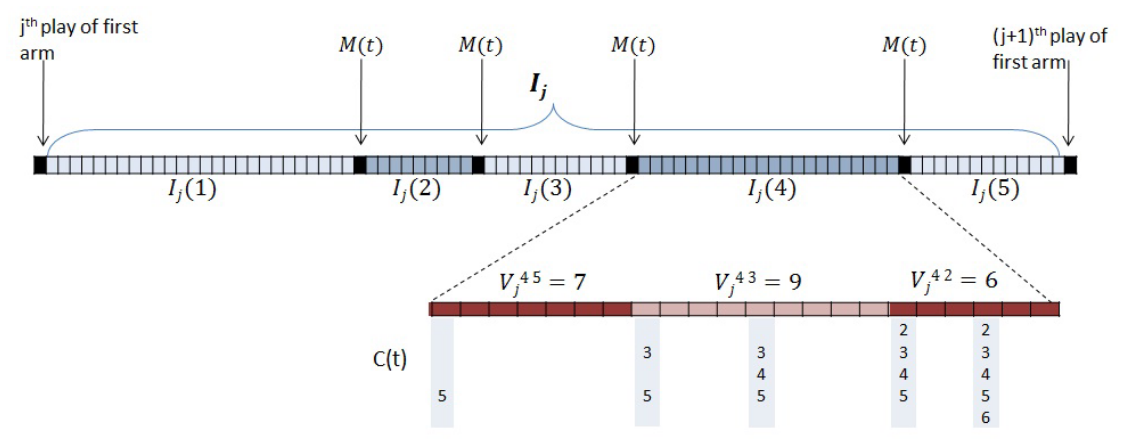
\includegraphics[width=\textwidth]{./figure/TS_proof.png}
\end{figure}

Where the `first arm' in the figure representing to the best arm $a^*$. The saturated set $C(\tau)$ is defined as at time $\tau$, if an arm $a\neq a^*$ has been selected more than $l_i=\dfrac{24\log t}{\Delta_a^2}$, then $a\in C(\tau)$, otherwise $a\notin C(\tau)$.

The seperate points are defined as an event $M(\tau)$. If $M(\tau)$ holds, then time $\tau$ is a seperate point. $\theta_{a}(\tau)$ is the sample for action $a$ at time $\tau$ from the Beta distribution, and the seperate event is defined as
$$M(\tau)=\I\left\{\theta_{a^*}(\tau)\max_{a\in C(\tau)}Q(a)+\dfrac{\Delta_a}{2}\right\}$$
The seperate points seperate the trials into intervals $I_j(1),\ldots,I_j(\gamma_j)$. Where $\gamma_j$ is the number of intervals. \\
Since a saturated arm $a$ can be played at step $\tau$ only if $\theta_a(\tau)>\theta_{a^*}(\tau)$. Saturated arm $a$ can be played at a time step $\tau\not\in I_j(\ell), \forall \ell, j$ (i.e., at a time step $\tau$ where $M(\tau)$ holds) only if $\theta_{a}(\tau) > Q(a) + \dfrac{\Delta_a}{2}$. Thus an event $E(\tau)$ is defined as
$$E(\tau)=\I\left\{\theta_{a}(\tau)\in\left[Q(a)-\dfrac{\Delta_a}{2},Q(a)+\dfrac{\Delta_a}{2}\right],\forall a\in C(\tau)\right\}$$
So the number of plays of saturated arms in interval $I_j$ is at most
$$\sum_{\ell=1}^{\gamma_j+1}|I_j(\ell)|+\sum_{\tau\in I_j}I(\overline{E(\tau)})$$
Also, define the number of saturated arm is played at each time step: let $V_j^{\ell,a}$ denote the number of steps in $I_j(\ell)$, for which $a$ is the best saturated arm:
$$V_{j}^{\ell,a}=\left|\left\{t\in I_j(\ell):Q(a)=\max_{a'\in C(\tau)}Q(a')\right\}\right|$$
And it could be proved that the expected regret due to playing saturated arms in interval $I_j$ is bounded as
\begin{align*}
\E\left[\R(I_j)\right] &\leq \E\left[\sum_{\ell=1}^{\gamma_j+1}\sum_{a|\Delta_a>0}3\Delta_aV_k^{\ell,a}\right]+2\E\left[\sum_{\tau\in I_j}\I(\overline{E_{\tau}})\right] \\
&\leq \E\left[\sum_{\ell=1}^{\gamma_j+1}|I_j(\ell)|\cdot\Delta_{\max}\right] + 2\sum_{\tau}P(\overline{E_{\tau}})
\end{align*}
Where $\Delta_{\max}=\max\limits_{a|\Delta_a>0}\Delta_a$ and $\Delta_{\min}=\min\limits_{a|\Delta_a>0}\Delta_a$. And $N$ is the number of arms of the bandit. \\
As $t\to\infty$, the constant form could be ignored, so above all, we have proved that the upper bound of the regret is
\begin{align*}
\lim_{t\to\infty} L_t &= \sum_j\E\left[\R(I_j)\right] \\
&\leq 1152\log t\left(\sum_{a|\Delta_a>0}\dfrac{1}{\Delta_a^2}\right)^2 + 288\log t\sum_{a|\Delta_a>0}\dfrac{1}{\Delta_a^2} + 48\log t\sum_{a|\Delta_a>0}\dfrac{1}{\Delta_a} + 192N\sum_{a|\Delta_a>0}\dfrac{1}{\Delta_a^2} + 96(N-1) + 8(N-1) \\
&\leq \log t\cdot \dfrac{\Delta_{\max}}{\Delta_{\min}^3}\cdot\left(\sum_{a|\Delta_a>0}\dfrac{1}{\Delta_a^2}\right)^2 \qquad\qquad\qquad\text{(Ignore constants)} \\
\Rightarrow \lim_{t\to\infty} L_t &\leq \log t\cdot \dfrac{\Delta_{\max}}{\Delta_{\min}^3}\cdot\left(\sum_{a|\Delta_a>0}\dfrac{1}{\Delta_a^2}\right)^2
\end{align*}
Reference: \href{https://arxiv.org/abs/1111.1797}{\textit{Analysis of Thompson Sampling for the Multi-armed Bandit Problem}}

\newpage